\section{Neuron Network}

% a 2 layer neuron network
\begin{figure}[h]
    \begin{center}
    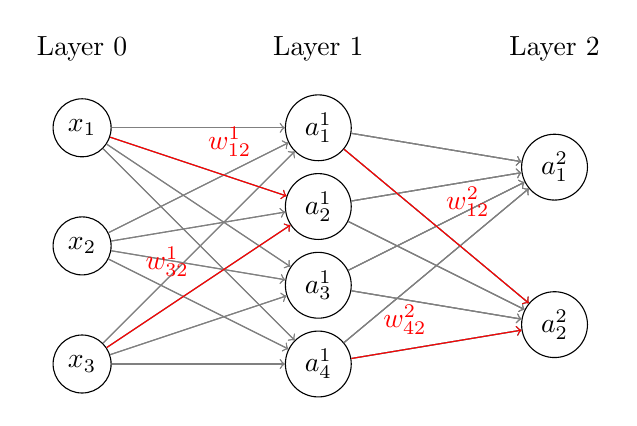
\begin{tikzpicture}
        % layer 0: input layer
        \begin{scope}[name prefix=layer0-]
            \node at (0, 0) {Layer 0};
            \node[circle, draw] (1) at (0, -1) {$x_1$};
            \node[circle, draw] (2) at (0, -2.5) {$x_2$};
            \node[circle, draw] (3) at (0, -4) {$x_3$};
        \end{scope}

        % layer 1
        \begin{scope}[name prefix=layer1-]
            \node at (3, 0) {Layer 1};
            \node[circle, draw] (1) at (3, -1) {$a^1_1$};
            \node[circle, draw] (2) at (3, -2) {$a^1_2$};
            \node[circle, draw] (3) at (3, -3) {$a^1_3$};
            \node[circle, draw] (4) at (3, -4) {$a^1_4$};
        \end{scope}

        % layer 2
        \begin{scope}[name prefix=layer2-]
            \node at (6, 0) {Layer 2};
            \node[circle, draw] (1) at (6, -1.5) {$a^2_1$};
            \node[circle, draw] (2) at (6, -3.5) {$a^2_2$};
        \end{scope}

        % weights
        \foreach \x in {1, 2, 3} {
            \foreach \y in {1, 2, 3, 4} {
                \foreach \z in {1, 2} {
                    \draw[gray, ->] (layer0-\x) -- (layer1-\y);
                    \draw[gray, ->] (layer1-\y) -- (layer2-\z);
                }
            }
        }
        \draw (layer0-1) edge[red, ->] node[auto] {$w^1_{12}$} (layer1-2);
        \draw (layer0-3) edge[red, ->] node[auto] {$w^1_{32}$} (layer1-2);
        \draw (layer1-1) edge[red, ->] node[auto] {$w^2_{12}$} (layer2-2);
        \draw (layer1-4) edge[red, ->] node[auto] {$w^2_{42}$} (layer2-2);
    \end{tikzpicture}
    \end{center}
    \caption{A 2 Layer Neuron Network}
\end{figure}

\subsection{Notations}
\begin{description}
    \item[$L$] output layer.
    \item[$n_l$] number of neurons in layer $l$. In particular, $n_0 = n$.
    \item[$w^l_{ij}$] weight from the $i$-th neuron in the layer $l-1$ to the $j$-th neuron in the layer $l$.
    \item[$b^l_j$] bias of the $j$-th neuron in layer $l$.
    \item[$a^l_j$] activation of the $j$-th neuron in layer $l$.
    \item[$z^l_j$] raw output of the $j$-th neuron in layer $l$.
    \item[$\sigma^l_j$] activation function of the $j$-th neuron in layer $l$.
    \item[$w^l$] weight matrix connecting layer $l-1$ to layer $l$, i.e. $(w^l_{ij})$, of dimension 
    $(n_{l-1},\ n_l)$.
    \item[$b^l$] bias vector of layer $l$, i.e. $(b^l_j)$, of dimension $(1, n_l)$.
    \item[$z^l$] raw output vector of layer $l$, of dimension $(1, n_l)$.
    \item[$a^l$] activation vector of layer $l$, of dimension $(1, n_l)$.
    \item[$\sigma^l$] activation function vector of layer $l$, of dimension $(1, n_l)$.
\end{description}

Some basic equations:

\begin{align}
    z^0_j &= a^0_j = x_j\\
    z^l_j &= \sum_k a^{l-1}_{k} w^l_{kj} + b^l_j\quad\forall~l\geq 1\\
    a^l_j &= \sigma^l_j(z^l_j)
\end{align}
The corresponding matrix forms are:

\begin{align}
    z^0 &= a^0 = \V{x} = (x_1, x_2, \ldots, x_{n})\\
    z^l &= a^{l-1} w^l + b^l\\
    a^l &= \sigma^l(z^l)
\end{align}

For a single input example \V{x}, the cost function $C$ should only directly depend on the output layer $L$,
for example $C$ is the square loss function:
\begin{equation}\label{nn_square_loss}
    C = \frac{1}{2} ||a^L - y||^2_2
\end{equation}
For a collection of examples, the cost function is the average cost on those examples:
\begin{equation}
    C = \frac{1}{m} \sum_{i=1}^m C(\V{x}_i)
\end{equation}

\subsection{Backpropagation}
First let's consider the case with a single input example. Let $\delta^l_j$ be the error in the $j$-th neuron
in the $l$-th layer, i.e.
\begin{equation}\label{delta_l_j}
    \delta^l_j = \pfrac{C}{z^l_j}
\end{equation}

For the output layer $L$, by definition we have:
\begin{align*}
    \delta^L_j &= \pfrac{C}{z^L_j}\\
               &= \sum_k \pfrac{C}{a^L_k} \pfrac{a^L_k}{z^L_j}\\
               &= \pfrac{C}{a^L_j} \pfrac{\sigma^L_j(z^L_j)}{z^L_j}\\
               &= \pfrac{C}{a^L_j}\cdot (\sigma^L_j)'(z^L_j)
\end{align*}
That is,
\begin{equation}
    \delta^L = \nabla_{a^L}C \odot (\sigma^L)'(z^L)
\end{equation}
For example, when $C$ is the square loss~\eqref{nn_square_loss}, $\nabla_{a^L}C = a^L - y$.
\par
We can write $\delta^l$ in terms of $\delta^{l+1}$ as following:
\begin{align*}
    \delta^l_j &= \pfrac{C}{z^l_j}\\
               &= \sum_k \pfrac{C}{z^{l+1}_k} \pfrac{z^{l+1}_k}{z^l_j}\\
               &= \sum_k \delta^{l+1}_k \sum_r \pfrac{a^l_r}{z^l_j} w^{l+1}_{rk}\\
               &= \sum_k \delta^{l+1}_k (\sigma^l_j)'(z^l_j) w^{l+1}_{jk}\\
               &= {\left(\delta^{l+1} \T{(w^{l+1})}\right)}_{j} (\sigma^l_j)'(z^l_j)
\end{align*}
Its corresponding matrix form is:
\begin{equation}
    \delta^l = \left(\delta^{l+1} \T{(w^{l+1})}\right) \odot (\sigma^l)'(z^l)
\end{equation}

Now, let's compute \pfrac{C}{b^l_j}:
\begin{align*}
    \pfrac{C}{b^l_j} &= \sum_k \pfrac{C}{z^l_k} \pfrac{z^l_k}{b^l_j}\\
                     &= \sum_k \delta^l_k \pfrac{b^l_k}{b^l_j}\\
                     &= \delta^l_j
\end{align*}
In shorthand, it can be rewritten as:
\begin{equation}
    \pfrac{C}{b} = \delta
\end{equation}

Similarly, we can compute \pfrac{C}{w^l_{ij}}:
\begin{align*}
    \pfrac{C}{w^l_{ij}} &= \sum_k \pfrac{C}{z^l_k} \pfrac{z^l_k}{w^l_{ij}}\\
                        &= \sum_k \delta^l_k \sum_r \pfrac{(a^{l-1}_r w^l_{rk} + b^l_k)}{w^l_{ij}}\\
                        &= \sum_k \delta^l_k a^{l-1}_i \delta_{kj}\\
                        &= a^{l-1}_i \delta^l_j
\end{align*}
In shorthand, it can be rewritten as:
\begin{equation}
    \pfrac{C}{w} = a_{\text{in}}\delta_{\text{out}}
\end{equation}

For simplicity, let's assume that all the activation functions are the same, i.e. $\sigma^l_i = \sigma$, then 
we can write the pseudocode of backpropagation algorithm easily as the following:

\begin{algorithm}
    \caption{Backpropagation}\label{backpropagation}
    \begin{algorithmic}[1]
        \Require $\V{x} = (x_1, x_2, \ldots, x_n)$
        \For{$l = 1$ \algorithmicto $L$}
            \State Compute $z^l = a^{l-1} w^l + b^l$ and $a^l = \sigma(z^l)$.
        \EndFor
        \State Compute $\delta^l = \nabla_{a^L}C \odot \sigma'(z^L)$\Comment{$\nabla_{a^L}C = a^L - y$ if $C$ 
        is square loss.}
        \For{$l=L-1$ \algorithmicto $1$}
            \State Compute $\delta^l = \left(\delta^{l+1} \T{(w^{l+1})}\right) \odot \sigma'(z^l)$
        \EndFor
        \Ensure $\pfrac{C}{w^l_{ij}} = a^{l-1}_i \delta^l_j$ and $\pfrac{C}{b^l_j} = \delta^l_j$.
    \end{algorithmic}
\end{algorithm}

We are now ready to do the vectorization. Let $\V{x}^i$ and $y^i$
be the $i$-th example and its output respectively, let
\begin{align*}
    X &= {(\V{x}^1; \ldots; \V{x}^m)}_{m \times n}\\
    Y &= {(y^1; \ldots; y^m)}_{m \times n_L}
\end{align*}
the input matrix. 
Let $z^{i, l}, a^{i, l}, \delta^{i, l}$ be the raw output, output, error vectors w.r.t.\ the
$i$-th example respectively. Let 
\begin{align*}
    Z^l &= {(z^{1, l}; \ldots; z^{m, l})}_{m \times n_l}\\
    A^l &= {(a^{1, l}; \ldots; a^{m, l})}_{m \times n_l}\\
    \Delta^l &= {(\delta^{1, l}; \ldots; \delta^{m, l})}_{m \times n_l}
\end{align*}
then we have:
\begin{align}
    Z^l &= A^{l-1} w^l + b^l\\
    A^l &= \sigma(Z^l)\\
    \Delta^L &= \nabla_{A^L}C \odot \sigma'(Z^L)\\
    \Delta^l &= \left(\Delta^{l+1} \T{(w^{l+1})}\right) \odot \sigma'(Z^l)
\end{align}
If $C = \frac{1}{m}\sum_{i=1}^m C(\V{x}_i)$, then
$$\pfrac{C}{b^l_j} = \operatorname{reduce\_mean}(\operatorname{col}_j(\Delta^l))$$
and
$$\pfrac{C}{w^l_{ij}} = \operatorname{reduce\_mean}(\operatorname{col}_i(A^{l-1}) \odot \operatorname{col}_j
(\Delta^l))$$

\subsection{Cost Functions}


\subsection{Regularizations}
\subsubsection{$L^1$ and $L^2$ Regularizations}

\subsubsection{Dropout}